\documentclass[letterpaper,11pt]{article}

\usepackage{geometry}
\usepackage{pslatex}
\usepackage{fancyhdr}
\usepackage{graphicx}
\usepackage{color}
\usepackage{enumitem} % for ordered list labels
\usepackage{amssymb} % for symbols
\usepackage{scrextend} % for indentation
\usepackage{tabto} % for tabs
\usepackage{amsmath} % for text in equation
\usepackage{forest, tikz} % to make forest

\graphicspath{ {./} }
\geometry{ margin = 1.0in }

%%% TODO modify these variables %%%
\def\homeworknum{7}
\def\myname{Harshit Jain}
\def\myaccessid{hmj5262}
\def\myrecitation{8}
%%%%

\pagestyle{fancy}
\lhead{{\bf CMPSC 465 Fall 2022}}
\chead{{\bf Assignment~\homeworknum}}
\rhead{{\bf \today}}

\newcounter{problemid}
%\stepcounter{problemid}
\def\newproblem{\clearpage\newpage{\bf Problem~\arabic{problemid}\stepcounter{problemid}}\hfill\fbox{\parbox{0.16\textwidth}{\bf Points:}}\par}

\setlength\parindent{0em}
\setlength\parskip{8pt}
\setlength{\fboxsep}{6pt}


\begin{document}

\framebox[\textwidth]{
	\parbox{0.96\textwidth}{
		\parbox{0.12\textwidth}{\bf Name:}\parbox{0.6\textwidth}{\myname}\\
		\parbox{0.12\textwidth}{\bf Access ID:}\parbox{0.6\textwidth}{\myaccessid}\\
		\parbox{0.12\textwidth}{\bf Recitation:}\parbox{0.6\textwidth}{\myrecitation}
	}
}


%% your solutions %%%

\newproblem
\textbf{Acknowledgements}
\begin{enumerate}[label=(\alph*)]
    \item I did not work in a group.
    \item I did not consult without anyone my group members.
    \item I did not consult any non-class materials.
\end{enumerate}


% PROBLEM 1
\newproblem
The given statement is \textbf{False}. If $f$ is a maximum $s-t$ flow in $G$, then $f$ need not to saturate every edge out of $s$ with flow.

\underline{Counter Example}:

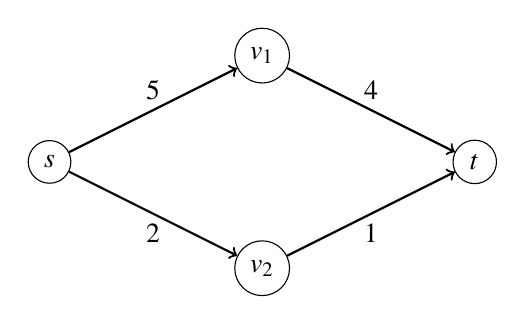
\begin{tikzpicture}[scale=0.9,auto=center]
	\node[circle, draw] (s) at (0, -1.5) {$s$};
	\node[circle, draw] (v_1) at (3, 0) {$v_1$};
	\node[circle, draw] (v_2) at (3, -3) {$v_2$};
	\node[circle, draw] (t) at (6, -1.5) {$t$};

	\draw[->, thick] (s) to node[anchor=south]{5} (v_1);
	\draw[->, thick] (v_1) to node[anchor=south]{4} (t);
	\draw[->, thick] (s) to node[anchor=north]{2} (v_2);
	\draw[->, thick] (v_2) to node[anchor=north]{1} (t);
\end{tikzpicture}

Here, the maximum flow on the upper branch will be $4$ since the bottleneck capacity for the path $s \Rightarrow v_1 \Rightarrow t$ is $4$.
The maximum flow on the lower branch will be $1$ since the bottleneck capacity for the path $s \Rightarrow v_2 \Rightarrow t$ is $1$.

Clearly, both the edges out of $s$ have flow value $f(e) < c_e$ where $c_e$ is the capacity of the edges coming out of node $s$. Therefore,
\[v(f) = \sum_{e \text{ out of } s} f(e) < \sum_{e \text{ out of } s} c_e = C\]

% PROBLEM 2
\newproblem


% PROBLEM 3
\newproblem

\end{document} 
